\documentclass[11pt]{article}
\usepackage[utf8]{inputenc}
\usepackage[margin=1in]{geometry}
\usepackage{siunitx,pgfplots,fancyhdr,enumitem,tikz,xparse,listings,graphicx,float}
\usepackage[T1]{fontenc}

\usepackage[colorlinks=true]{hyperref}

\lstset{language=Matlab}

%%Needed to properly display graphs
\pgfplotsset{width=10cm,compat=1.9}

\pagestyle{fancy}
\fancyhf{}
\lhead{Steven Glasford}
\chead{Homework 4}
\rhead{Page \thepage}

\title{Homework 4}
\author{Steven Glasford}
\date{\parbox{\linewidth}{\centering%
    %%Adds the last compiled date
    \today\endgraf\medskip
    Numerical Analysis\endgraf\medskip
    MATH-373}}

%%Creates a new symbol for plus and minus together
\newcommand{\rpm}{\sbox0{$1$}\sbox2{$\scriptstyle\pm$}
  \raise\dimexpr(\ht0-\ht2)/2\relax\box2 }

%%Creates a nice format for displaying the steps taken  
\newlist{steps}{enumerate}{1}
\setlist[steps, 1]{label = Step \arabic*:}

\ExplSyntaxOn
%%new command to round numbers
\newcommand*{\prlen}[1]{%
   % round to 1 digit:
    \pgfmathparse{round(10)/10.0}%
    %\pgfkeys{/pgf/number format/precision=1}
    %\pgfmathresult
    \pgfmathprintnumber[fixed, precision=2]{\pgfmathresult}
}
\ExplSyntaxOff

% Set the listings programming language
\lstset{language=Matlab}

\begin{document}

%% adds the title to the document
\maketitle
\pagebreak
%\tableofcontents

\section{Problem Statement}
We are going to check the claims of Estes Industries, which manufactures rocket engines for low-powered rockets.  For instance, Estes Industries manufactures a C11 engine, which should produce an average thrust of \SI{11}{N} and a total impulse of 5--10 \si{N.s}.  The letter in the engine name designates a class of engine that produces a certain impulse.  Table \ref{table:estes} lists some of the classes that Estes Industries manufactures, along with the associated range of total impulses.  The number in the name states the average thrust of the engine over its burn time.

	\begin{table}[h]
	\begin{center}
	\caption{Engine class and total impulse.}\label{table:estes}
	\smallskip
	\begin{tabular}{c|c}
	Class & Impulse (\si{N.s})\\\hline
	A & 1.25--2.5\\
	B & 2.5--5\\
	C & 5--10\\
	D & 10--20\\
	E & 20--40\\
	\end{tabular}
	\end{center}
	\end{table}
	
The website \url{www.thrustcurve.org} has tested many rocket engines, and it provides data for each engine as thrust (in Newtons) versus time (in seconds).  We will use this data to test the claims of the C11, D11, D12, and E12 engines.  First, impulse is defined as $$I = \int_{t_0}^{t_f} F(t)\,dt,$$ where $F(t)$ is the thrust as a function of time, $t_0$ is the start time, and $t_f$ is the final time.  Second, the average value of a function, $f(x)$, over the interval $[a,b]$ is defined as $$f_{ave} = \frac{1}{b-a}\int_a^b f(x)\,dx,$$ which we can use to compute the average thrust of each engine.  Note that since we only have data about the thrust, we will need to use the program \texttt{trapezoid\_data} to compute these integrals.

For each engine, complete the following steps.  I recommend writing a MATLAB function that performs these steps for a given engine, and then you can run the function for each engine.  I also recommend that the only input to this function be the variable \texttt{filename}, which contains the name of the file to be loaded.  The outputs would be the total impulse and the average thrust.

	\begin{enumerate}
	
	\item  Load the .mat file with the necessary data using the command \texttt{load(filename)}, where \texttt{filename} is a string containing the name of the file.  The .mat files for the engines are in a .zip files on the course website.  The \texttt{load} command will create a variable called \texttt{thrust\_data}, which will be loaded with the information for the rocket engine.  This variable will not appear in the Workspace window, but it will exist.  I suggest calling the variable in your M-file without a semicolon after you load it so that you can see what it looks like.  Determine the dimensions of \texttt{thrust\_data} using the \texttt{size} command.  For instance, to load the information for the C11 engine, use the command
	
		\texttt{load('C11\_thrust\_curve.mat');}
		
		though if you use the input \texttt{filename}, all you would use is
		
		\texttt{load(filename);}
		
		and the string would be the input to the function.
	
	\item  Plot the thrust data using the \texttt{plot} command.  Include a title and axis labels using the \texttt{title}, \texttt{xlabel}, and \texttt{ylabel} commands.  The \texttt{:} operate will be helpful.
	
	\item  Use \texttt{trapezoid\_data} to compute the total impulse and average thrust of the engine.
	
	\item  Plot the average thrust as a dashed horizontal line on the same plot as the thrust data.  The \texttt{hold} command will be needed for this.
	
	\item  Evaluate the claims of the engine designation.  If the engine designation is incorrect, what should it be?
	
	\end{enumerate}
	
Provide a subsection for each of the four engines that includes all of the information produced above.  The report must be typeset using \LaTeX\ and a hard copy should be submitted in class.  Be sure to follow the template for homework on the course website.


\section{Solution}

\begin{center}
\begin{tabular}{c|c|c}
     \emph{Engine Type}&\emph{Total Impulse}&\emph{Average Thrust} \\
     \hline
     C11 &8.7961&10.8593\\
     D11 &17.4895&9.4029\\
     D12 &16.8391&10.2055\\
     E12 &27.1359&11.1213
\end{tabular}
\end{center}

The plot for the \texttt{C11\_thrust\_curve.mat} can be found in figure \ref{fig:c11} on page \pageref{fig:c11}.

The plot for the \texttt{D11\_thrust\_curve.mat} can be found in figure \ref{fig:d11} on page \pageref{fig:d11}.

The plot for the \texttt{D12\_thrust\_curve.mat} can be found in figure \ref{fig:d12} on page \pageref{fig:d12}.

The plot for the \texttt{E12\_thrust\_curve.mat} can be found in figure \ref{fig:e12} on page \pageref{fig:e12}.

\medskip

All of the rocket designations seemed to be accurate, and would be able to be trust worthy, as they are all within the bounds provided earlier.


\section{Command-line Usage}
One program was written to produce the graphs in this document, then the graphs were exported to images and inserted into this document. To use this one file (the contents of which can be found in Code \ref{code:hw4}): 

\begin{verbatim}
>> hw4()
\end{verbatim}

\section{Code}

\lstinputlisting[caption={MATLAB Code to Solve the Problem}, label = {code:hw4}, frame=tb]{hw4.m}

\lstinputlisting[caption={MATLAB Code \texttt{trapezoid.m}}, label = {code:trapezoid},frame=tb]{trapezoid.m}

\lstinputlisting[caption={MATLAB Code \texttt{trapezoid\_data.m}}, label = {code:data},frame=tb]{trapezoid_data.m}

\lstinputlisting[caption={MATLAB Code \texttt{simpsons\_third.m}}, label = {code:simpson},frame=tb]{simpsons_third.m}

\newpage

\begin{figure}
    \centering
    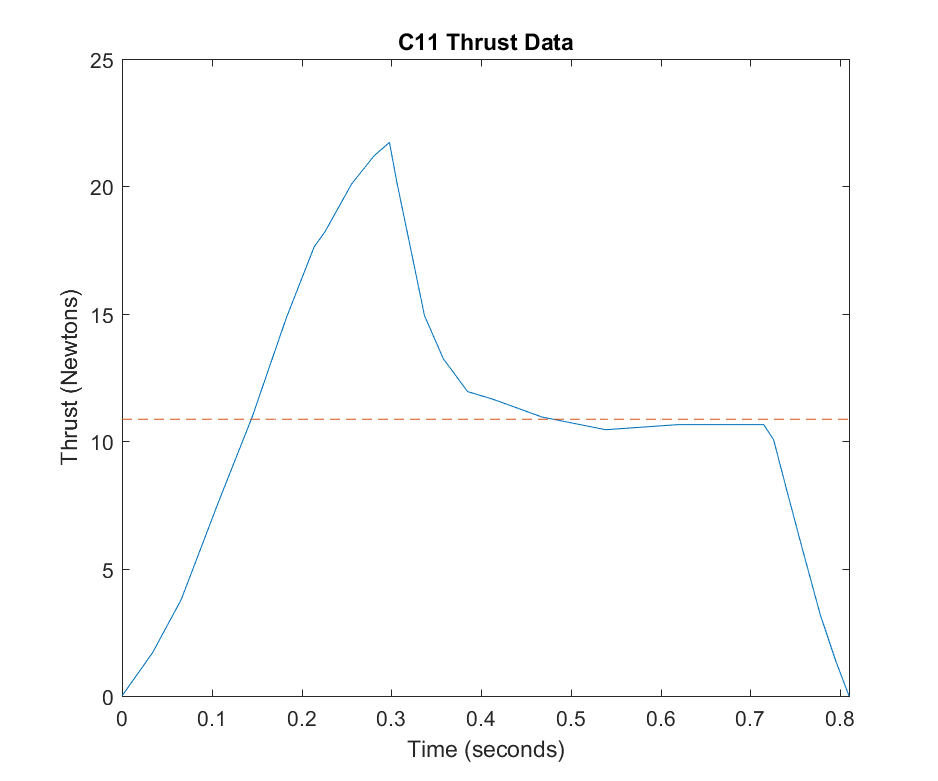
\includegraphics{c11.png}
    \caption{Graph for \texttt{C11\_thrust\_curve.mat}}
    \label{fig:c11}
\end{figure}

\begin{figure}
    \centering
    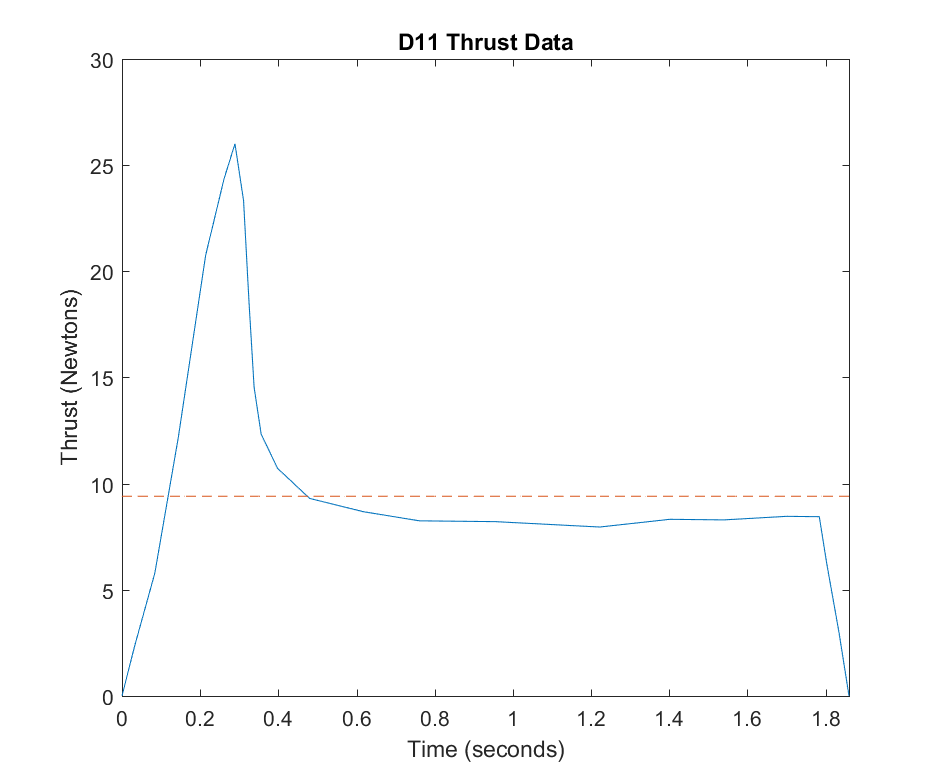
\includegraphics{d11.png}
    \caption{Graph for \texttt{D11\_thrust\_curve.mat}}
    \label{fig:d11}
\end{figure}

\begin{figure}
    \centering
    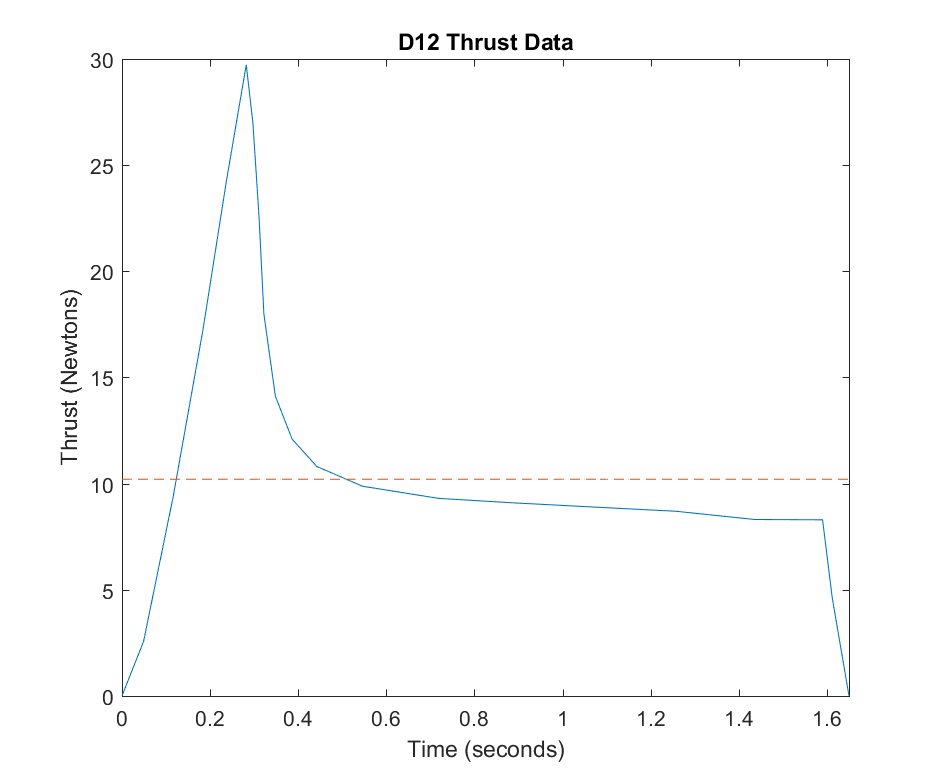
\includegraphics{d12.png}
    \caption{Graph for \texttt{D12\_thrust\_curve.mat}}
    \label{fig:d12}
\end{figure}

\begin{figure}
    \centering
    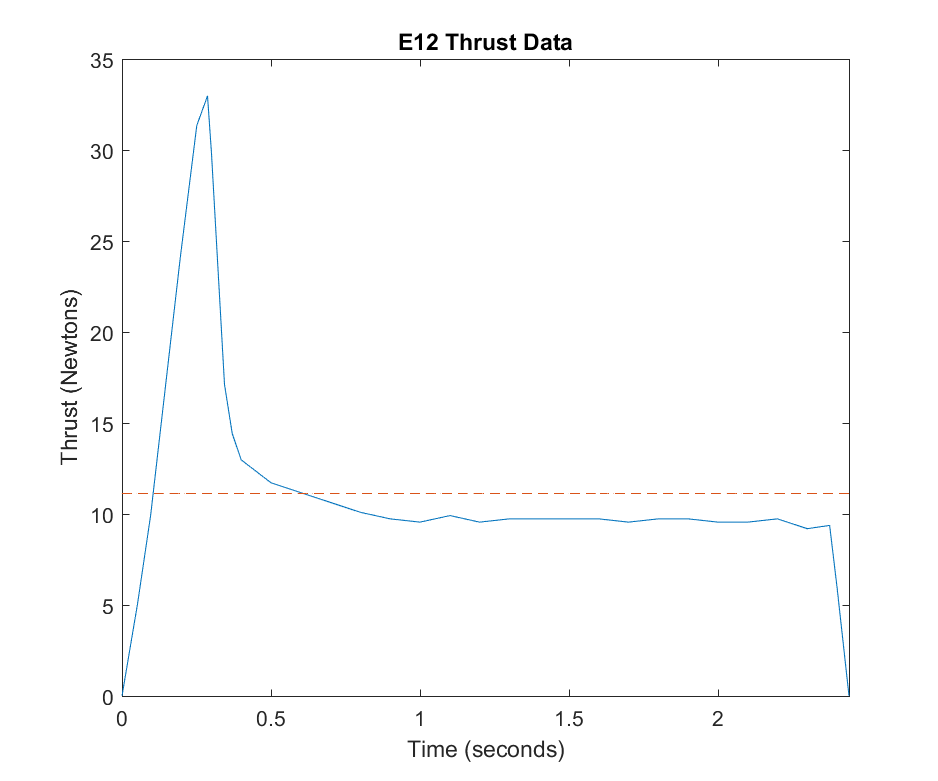
\includegraphics{e12.png}
    \caption{Graph for \texttt{E12\_thrust\_curve.mat}}
    \label{fig:e12}
\end{figure}

\end{document}